\documentclass[../00_main.tex]{subfiles}

\begin{document}

\section{Data Investigation}

In this section, I will use my program and the skills I learned during this
internship to explore the vertical structure of air pressure, as per my
supervisor's suggestion. I will show the tropopause zone, the vertical gradient
of the air temperature and explain why it is like it is, and the inverse
gradient caused by the ozone layer.

\subsection{The Troposphere and Tropopause}

The Troposphere is the lowest layer of the atmosphere -- starting on the 
surface it reaches an average height of 12 km. The air pressure in the 
troposphere decreases non--linearly as the height above the surface increases.
The temperature in the troposphere also generally decreases when the pressure
decreases. At the top of the troposphere, the temperature is -63\textdegree{}C
or about 210K \cite{tropopause}. The pressure range of the troposphere is about 
1000 hPa to 200 hPa according to \cite{pressure}.\newline

The boundary between the troposphere and the next layer of the atmosphere,
the stratosphere, is called the tropopause. The tropopause can be demarcated
by multiple factors. One factor is the inversion of the temperature gradient of
the troposphere, meaning that the temperature starts to increase with
a decrease in pressure, not to decrease like before \cite{tropopause}.
Another metric by which to define the tropopause is a sharp increase in
potential vorticity, a measure of the rotation of the air masses 
\cite{tropopause}. The third factor indicating the tropopause is the abrupt 
increase of the ozone mixing ratio. The ozone mixing ratio is a measure of how 
much ozone is part of the air by either mass or volume 
\cite{atmosphere}.\newline

To investigate these behaviors, I modified my plotting program to plot all
pressure levels of a certain variable for a specific date and time, and
position. The following subsections use these plots to explain the behavior
above. To be comparable, all plots are using the exact same data: M2I3NPASM
data for the 01.09.2019 at 12:00 for the position (40\textdegree{}N,
70\textdegree{}E).

\subsubsection{Air Temperature}

As stated above, the air temperature is expected to drop continuously as the
pressure decreases from 1000 hPa to about 200 hPa. After that, in the
tropopause, the temperature is expected to sharply increase. \figref{temp}
illustrates this behavior. On the $y$ axis the pressure is plotted in reversed
order, representing the decrease in pressure as the altitude increases. To
better show the changes in pressure, it is plotted using a $\log_{10}$ scale. 
The $x$ axis shows the temperature in Kelving ($K$).
\begin{figure}[H]
\center
    \fbox{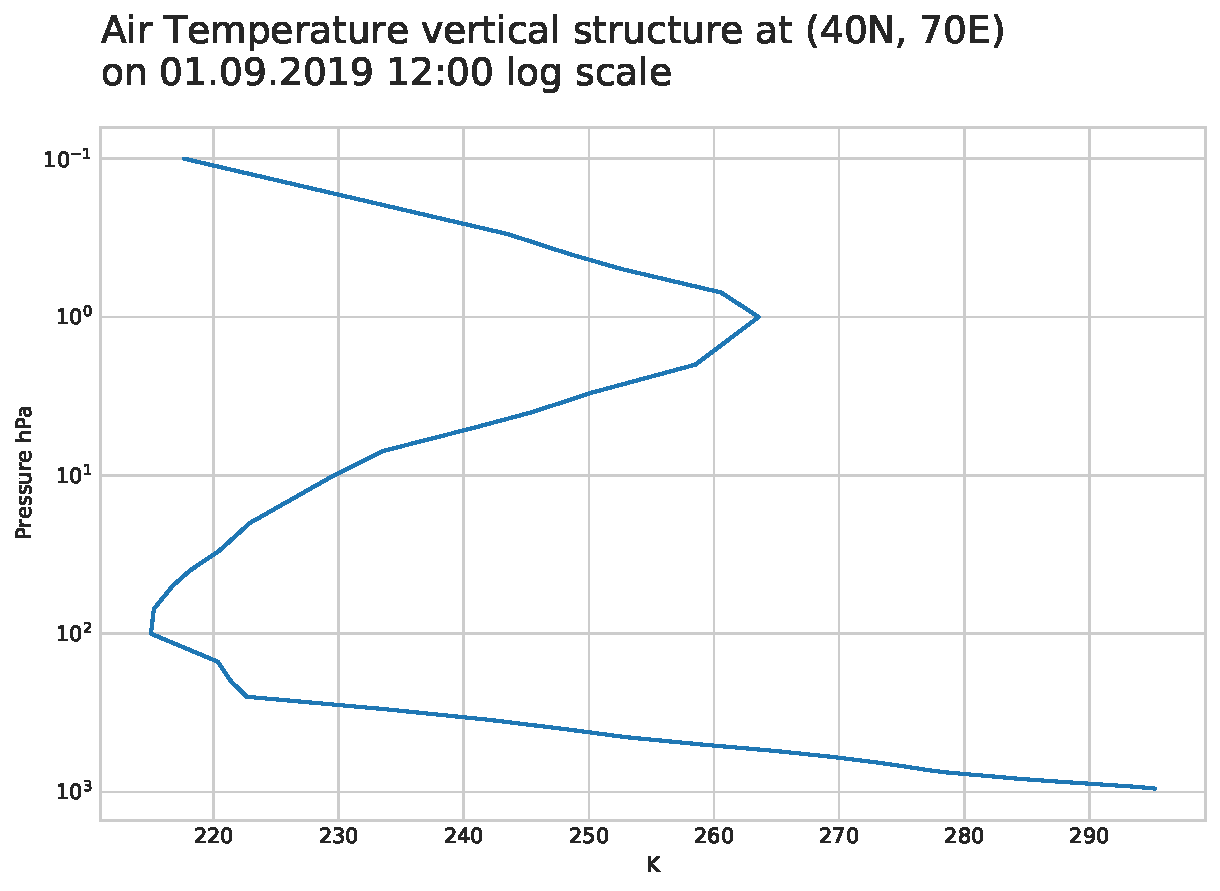
\includegraphics[width=\textwidth]{../graphics/temperature}}
    \vspace{-20pt}
    \caption{Air Temperature by Air Pressure}
    \label{temp}
\end{figure}
We see that after about 200 hPa the temperature decreases to about 210K and
then sharply increases, as expected for the tropopause. The increase in
temperature around 1 hPa is probably due to the ozone layer in the stratosphere
seen in \figref{ozone}.

\subsubsection{Potential Vorticity}

The second indicator of the tropopause is a sharp increase in the potential
vorticity that should occur around 200 hPa. The satellite data includes Ertel's
Potential Vorticity (EPV), which shall be used here. \figref{epv} illustrates 
the sharp increase in potential vorticity. The $y$ axis shows the pressure in
reverse in a $\log_{10}$--based scale to make the transition more clear. The
$x$ axis shows Ertel's Potential Vorticity.
\begin{figure}[H]
\center
    \fbox{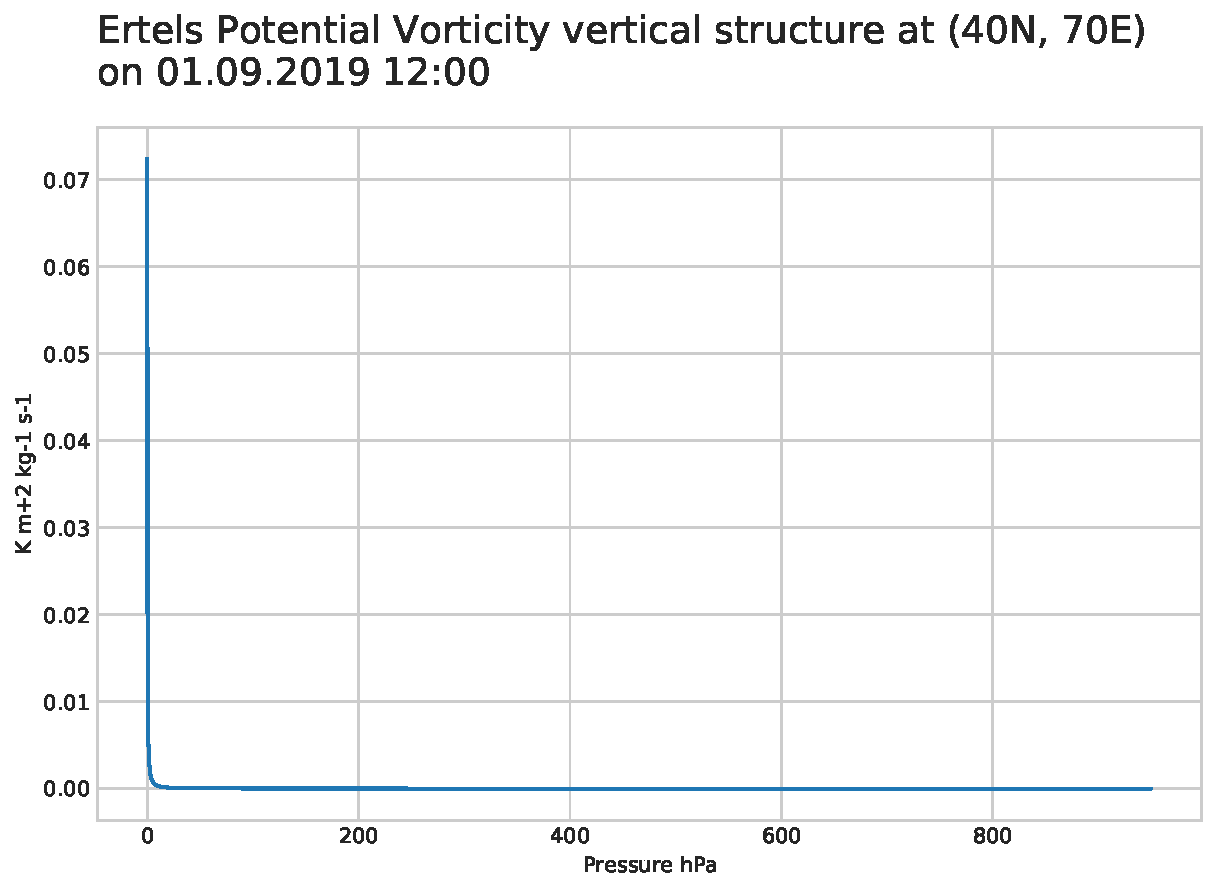
\includegraphics[width=\textwidth]{../graphics/epv}}
    \vspace{-20pt}
    \caption{Ertel's Potential Vorticity by Air Pressure on a $\log_{10}$ scale}
    \label{epv}
\end{figure}

\subsubsection{Ozone Mixing Ratio}

The third marker of the tropopause is the increasing ozone mass mixing ratio,
represented by the O3 variable of the M2I3NPASM dataset. The ratio increases
most in the stratosphere though, especially in the ozone layer. In 
\figref{ozone} we see that as the pressure approaches approximately 10 hPa, the 
ozone mass mixing ratio increases sharply. This is the ozone layer in the 
stratosphere. \figref{ozone} again has the pressure on the $y$ axis, inverted
and $\log_{10}$--based. The ozone mass mixing ratio is plotted on the $x$ axis.
\begin{figure}[H]
\center
    \fbox{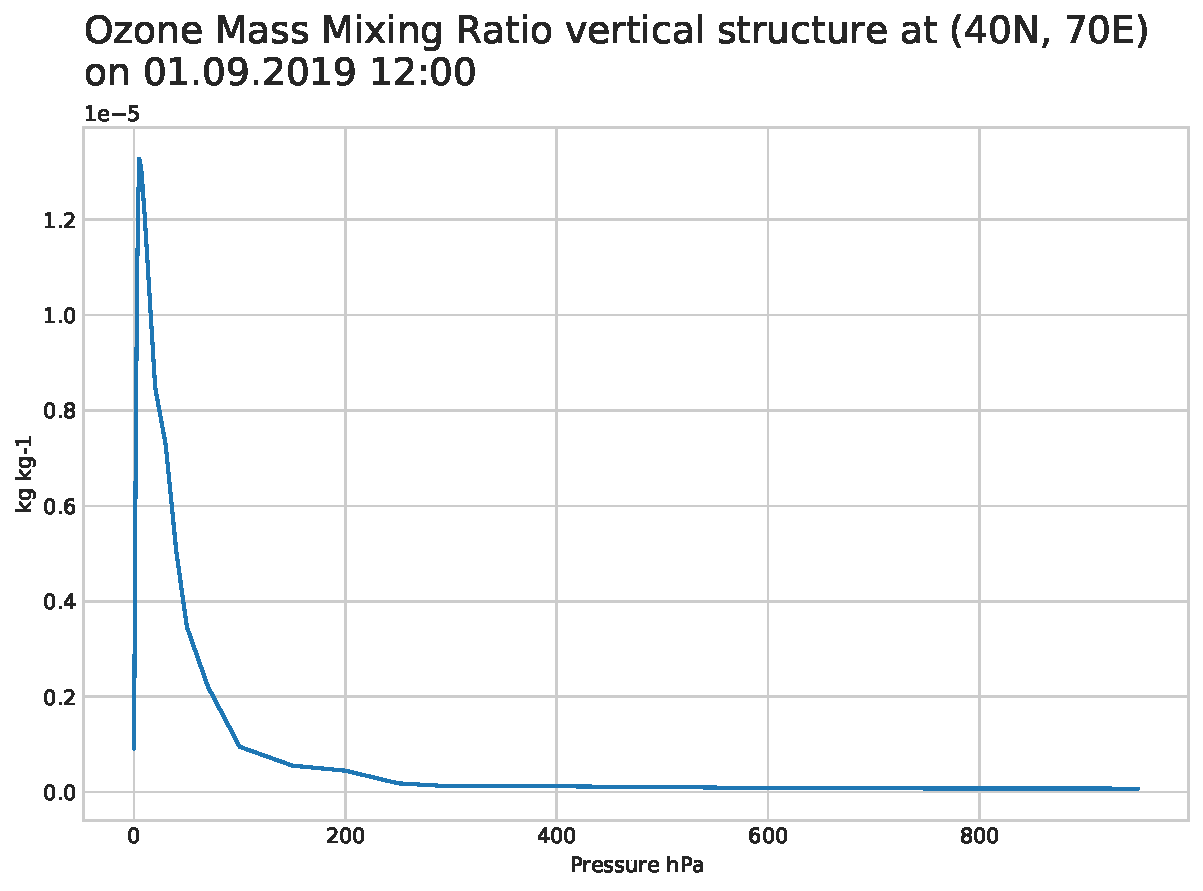
\includegraphics[width=\textwidth]{../graphics/ozone}}
    \vspace{-20pt}
    \caption{Ozone Mass Mixing Ratio by Air Pressure on a $\log_{10}$ scale}
    \label{ozone}
\end{figure}
\figref{ozone} supports our assumptions about the ozone mass mixing behavior in
the tropopause.

\subsection{Reasons for Temperature Inversion}

According to \cite{inversion}, the temperature inversion in the tropopause is caused by
heating as a result of sunlight absorption by molecules and aerosols in the
tropopause.\\
As \figref{ozone} showed, the ozone mass mixing ratio increases sharply as the
pressure decreases to about 10 hPa. While most ozone is contained in the
stratosphere, where it absorbs ultraviolet radiation, some is also contained
in the troposphere, as shown. Ozone absorbs ultraviolet radiation and heat is
resealed in the process \cite{ozone}.
The ozone in the troposphere might absorb ultraviolet light that got through
the troposphere and release heat in the process which in turn warms up the
tropopause.

\end{document}
